
%(BEGIN_QUESTION)
% Copyright 2006, Tony R. Kuphaldt, released under the Creative Commons Attribution License (v 1.0)
% This means you may do almost anything with this work of mine, so long as you give me proper credit

%In any automated (controlled) system, there is a {\it process variable}, a {\it setpoint}, and a {\it manipulated variable}.  There is also something called a {\it load}, which influences how well the control system is able to maintain setpoint.  Provide a general description for a ``load,'' and then identify the load(s) in each of the following manually-controlled processes:

I alle reguleringssystem er det en Prosessvariabel (PV), et settpunkt (SP) og en manipulerendevariabel (MV). Det er også noe kalt last som er med på å avgjøre hvor godt systemet holder settpunktet. Gi en generell beskrivelse av last og identifiser lastene i eksemplene nedenfor. 


\vskip 30pt

\noindent
{\bf Example 1:} Temperaturreguleringssystem % Temperature control application

$$\includegraphics[width=15.5cm]{i01453x01.eps}$$

\vskip 30pt

\filbreak
\noindent
{\bf Example 2:} Nivåreguleringssystem % Level control application

$$\includegraphics[width=15.5cm]{i01453x02.eps}$$

\vskip 30pt

\filbreak
\noindent
{\bf Example 3:} Strømningsreguleringssystem % Flow control application

$$\includegraphics[width=15.5cm]{i01453x03.eps}$$

\vskip 30pt

\filbreak
\noindent
{\bf Example 4:} Temperaturreguleringssystem % Temperature control application

$$\includegraphics[width=15.5cm]{i01453x04.eps}$$

\vskip 20pt \vbox{\hrule \hbox{\strut \vrule{} {\bf Suggestions for Socratic discussion} \vrule} \hrule}

\begin{itemize}
\item{$\bullet$} Explain why ambient air temperature is considered a {\it load} to process example \#4, but the insulation thickness on the heat exchanger is not.
\medskip

\underbar{file i01453}
%(END_QUESTION)





%(BEGIN_ANSWER)

A {\it load} is any variable in a process (besides the manipulated variable) that has influence over the process variable being controlled.

\vskip 10pt

Note: the following answers are not exhaustive.  In other words, there may be more loads than what is listed here for each process!

\begin{itemize}
\item{$\bullet$} Example 1: ambient air temperature
\item{$\bullet$} Example 2: incoming flow rate
\item{$\bullet$} Example 3: upstream and downstream pressures
\item{$\bullet$} Example 4: steam flow rate, steam temperature
\medskip

%(END_ANSWER)





%(BEGIN_NOTES)

Students may be tempted to list process {\it constants} (such as vessel volume, heat exchanger tube thickness, etc.) as loads because they do impact the process dynamics.  However, the term ``load'' is typically reserved for some {\it variable} that has impact over the process, and is thus liable to change over time in such a way to challenge the loop controller.

To put this in different terms, the need to change setpoints, and the existence of variable loads in a process, both {\it justify} the presence of a controller.  If we were faced with a process never needing a different setpoint, and devoid of variable loads, there would be no need to place a control loop in it!  We could simply set a manually-actuated control valve where we wanted it to be, and leave it in that position forever!

\vfil \eject

\noindent
{\bf Prep Quiz:}

The definition of a {\it load} with regard to process control loops is:

\begin{itemize}
\item{$\bullet$} The time lag between a change in output and a change seen in the PV
\vskip 5pt 
\item{$\bullet$} The value at which the control system attempts to stabilize the PV over time
\vskip 5pt 
\item{$\bullet$} A device that dissipates energy in a circuit, as opposed to sourcing energy to the circuit
\vskip 5pt 
\item{$\bullet$} The multiplication factor of a process, measured from output to input
\vskip 5pt 
\item{$\bullet$} A drain of energy on a system, causing it to operate inefficiently
\vskip 5pt 
\item{$\bullet$} A variable affecting the PV, that is itself unregulated by the control system
\medskip



%INDEX% Control, basics: load (definition)

%(END_NOTES)


